\documentclass[
  11pt,
  fleqn
]{article}
% [fleqn] left-aligns all equations

% fonts

\usepackage[T1]{fontenc} % Apparently this
% https://tex.stackexchange.com/questions/287312/font-not-loadable-metric-data-not-found-or-bad
\usepackage[full]{textcomp}
\usepackage[final,expansion=alltext,nopatch=footnote]{microtype}
\usepackage{csquotes} % suppress warning from `babel`
\usepackage[english]{babel}
\usepackage[fleqn]{mathtools}
\usepackage[cal=boondoxo]{mathalpha} % mathcal

\usepackage{amsthm} % gives proof environment:
% https://www.overleaf.com/learn/latex/Theorems_and_proofs

\usepackage{newtxtext}
% \usepackage{txfonts} % See
% https://tex.stackexchange.com/questions/444243/symbols-not-showing-up

% These need to be after newtxtext
\usepackage[varqu,varl]{inconsolata} % sans serif typewriter
% \usepackage{cabin} % sans serif - ugly

\usepackage[bigdelims,vvarbb]{newtxmath} % bb from STIX % "should be
% loaded AFTER the text font" -
% https://mirrors.mit.edu/CTAN/fonts/newtx/doc/newtxdoc.pdf

% geometry of the page

\usepackage[
  % top=1in,
  % bottom=1in,
  % left=1in,
  % right=1in
]{geometry}

% paragraph spacing

\setlength{\parindent}{0pt}
\setlength{\parskip}{1.5ex plus 0.4ex minus 0.2ex}

% useful packages

% \usepackage{natbib} % incompatible with BibLaTeX
\usepackage{epsfig}
\usepackage{url}
\usepackage{bm}
\usepackage{blindtext}

% Leon additions

\usepackage{enumitem} % allows for enumerate[resume]

\usepackage{booktabs}

\usepackage[
  style=authoryear-comp,
  natbib=true,
  % refsection=chapter,
  url=false,
  doi=true,
  isbn=false,
  date=year %
  % https://tex.stackexchange.com/questions/55780/disable-month-in-biblatex-bibliography
]{biblatex} % natbib=true allows \citep
% Clear "visited on"
% https://tex.stackexchange.com/questions/400384/how-to-disable-biblatex-showing-visited-on-on-the-references
\AtEveryBibitem{
  \clearfield{urlyear}
  \clearfield{urlmonth}
  \clearfield{eprint} % remove PMID %
  % https://tex.stackexchange.com/questions/250784/removing-eprint-and-eprinttype-in-citation-notes
}

\usepackage{graphicx}
% ensures figures stay in their section
% https://tex.stackexchange.com/questions/279/how-do-i-ensure-that-figures-appear-in-the-section-theyre-associated-with
\usepackage[section]{placeins}

% Section formatting using titlesec
\usepackage{titlesec}
\titleformat*{\section}{\singlespacing\sffamily\Large}
\titleformat*{\subsection}{\singlespacing\sffamily\large}
% \titleformat*{\subsubsection}{\itshape}
\titleformat*{\paragraph}{\itshape}
\titleformat{\chapter}{\singlespacing\sffamily\Huge}{{\thechapter}}{1em}{}

% center figures by default
\makeatletter
\g@addto@macro\@floatboxreset\centering
\makeatother
% italic figure captions
\usepackage[format=plain,
  textfont=it,
]{caption}

% simple TO DO and comment macros
\usepackage[
  % https://tex.stackexchange.com/questions/4503/how-do-i-specify-color-in-rgb-using-hypersetup-in-hyperref
  dvipsnames,svgnames,x11names
]{xcolor}
\newcommand\todo[1]{\textcolor{orange}{[#1]}}% simple TO DO macro
\newcommand\comment[1]{\textcolor{red}{[#1]}}

\usepackage{url}
\usepackage[
  hidelinks,
  pdfa % Required for valid pdf/a output:
  % https://tex.stackexchange.com/questions/431022/pdf-a-validation-problem-the-f-key-is-missing
]{hyperref}
\hypersetup{
  % colorlinks,
  % linkcolor=RoyalBlue4,
  % citecolor=PaleVioletRed4,
  % urlcolor=Firebrick4
}

\newcommand{\indsim}{\overset{\mathrm{ind}}{\sim}}
% https://tex.stackexchange.com/questions/60545/should-i-mathrm-the-d-in-my-integrals
\newcommand*\diff{\mathop{}\!\mathrm{d}}
\newcommand*\Diff[1]{\mathop{}\!\mathrm{d^#1}}
\newcommand{\e}{\mathrm{e}}
\newcommand{\E}{\mathrm{E}}
\renewcommand{\P}{\mathrm{P}}
\newcommand{\N}{\mathrm{N}}
\newcommand{\diag}{\mathrm{diag}}
\newcommand{\ave}{\mathrm{ave}}
\newcommand{\Var}{\mathrm{Var}}
\newcommand{\Cov}{\mathrm{Cov}}
\newcommand{\cov}{\mathrm{cov}}
\newcommand{\sd}{\mathrm{sd}}
\newcommand{\var}{\mathrm{var}}
\newcommand{\corr}{\mathrm{corr}}
\renewcommand\vec{\boldsymbol}

% Overlap-specific
\newcommand{\rank}{R}
\newcommand{\rmax}{m}
\newcommand{\rgap}{r^\text{gap}}
\newcommand{\Ngap}{N_1^\text{gap}}
\newcommand{\pigap}{\pi_1^\text{gap}}

% For appearance of block matrices
% https://tex.stackexchange.com/questions/495903/horizontal-and-vertical-lines-in-pmatrix
\renewcommand{\arraystretch}{1.5}

% Theorem-type environments
\newtheorem{definition}{Definition}[section]
\newtheorem{result}[definition]{Result}
\newtheorem{claim}[definition]{Claim}

% From Datta template
% https://github.com/bibekanandadatta/JHU-Dissertation-Template

\usepackage{setspace}                         % sets space between lines

%%%% JH Library requirement (DO NOT CHANGE)
\def\GlobalMargin{1.0in}                      % margin on all sides
% \def\PrintingOffset{0.5in}                  % additional left
% margin for the printed copy
\def\PrintingOffset{0.0in}
\def\MainTextSpacing{\singlespacing}        % double-spaced main text
% \def\MainTextSpacing{}
\def\CaptionStretch{1.1}                    % to match 2x spacing
% \def\CaptionStretch{1.0}

\captionsetup{font={stretch=\CaptionStretch}}

\geometry{
  letterpaper,
  margin=\GlobalMargin,
  bindingoffset=\PrintingOffset,
  nomarginpar,
  % includehead,
  % headheight=\HeaderHeight,
  % headsep=\HeaderSpace,
  includefoot,
  heightrounded
}

%%%% BIBLIOGRAPHY ITEMS
\def\BibTextSpacing{\onehalfspacing}         % single-spaced bibliography
% \def\BibTextSpacing{\singlespacing}         % single-spaced bibliography
\def\BibItemSpacing{\baselineskip}          % spacing between
% bibliographic items in reference

%%%% UNNUMBERED CHAPTERS, SECTION, and SUBSECTION COMMAND for ADDING to TOC
%% removes the 'Chapter #' title while keeping it listed in the TOC
\newcommand\chap[1]{%
  \chapter*{#1}%
  \markboth{#1}{}
\addcontentsline{toc}{chapter}{#1}}

%% removes the 'Section #' title while keeping it listed in the TOC
\newcommand\sect[1]{%
  \phantomsection
  \section*{#1}%
\addcontentsline{toc}{section}{#1}}

%% removes the 'Subsection #' title while keeping it listed in the TOC
\newcommand\subsect[1]{%
  \phantomsection
  \subsection*{#1}%
\addcontentsline{toc}{subsection}{#1}}

%% removes the 'Subsubsection #' title while keeping it listed in the TOC
\newcommand\subsubsect[1]{%
  \phantomsection
  \subsubsection*{#1}%
\addcontentsline{toc}{subsubsection}{#1}}

% Correct matrix for double spacing
% https://tex.stackexchange.com/questions/137004/matrix-within-equation/137009#137009
\makeatletter
\def\env@matrix{\hskip -\arraycolsep
  \let\@ifnextchar\new@ifnextchar
  \linespread{1}\selectfont
  \renewcommand{\arraystretch}{1.2}%
\array{*\c@MaxMatrixCols c}}
\makeatother

% Footnotes must be 2 points less than main text but larger than 8pt
\usepackage{footmisc}
\renewcommand{\footnotesize}{\fontsize{9pt}{11pt}\selectfont}

% For including CV
\usepackage{pdfpages}

% Generate PDF/A (archival format)
% https://webpages.tuni.fi/latex/pdfa-guide.pdf
\usepackage[a-1b,mathxmp]{pdfx}

\usepackage[
  nottoc % Don't include TOC in TOC
]{tocbibind}

% Redefine `abstract`s so they can be at the start of each chapter
% don't cause the page numbering to reset
% https://tex.stackexchange.com/a/4857
\newenvironment{myAbstract}{
  \rightskip.5in
  \leftskip.5in
  % \itshape
}{}

% For writing/planning purposes: show paragraph level in TOC
\setcounter{secnumdepth}{3}

\addbibresource{bibliography.bib}
\graphicspath{{fig/}}

\title{Guidance for clinicians in constructing ordinal outcomes and choosing
ordinal effect measures for clinical trials}
\author{Leon Di Stefano + Ordinal
Working Group}
\date{\today}

\begin{document}

\maketitle

\tableofcontents
\newpage

\section{Introduction}

Ordinal outcomes have become increasingly prominent in clinical
resarch, particularly following the COVID-19 pandemic, when ordinal
scales developed by the WHO and NIAID were used in prominent trials
of drugs repurposed to treat the disease \todo{cite}. They have also
been a popular choice in adaptive platform trials \todo{cite}.

Some advantages of ordinal outcomes are that they can
\begin{enumerate}
  \item Provide more information that binary outcomes, including
    composite outcomes, making study designs more sensitive and precise, and
    therefore more efficient and ethical

  \item Allow for the incorporation of intercurrent events into one's primary
    outcome, avoiding complexities of alternative estimand strategies like
    principal stratum estimands (particular for truncating events
    like death) while
    yielding more statistical efficiency than traditional binary
    composite outcomes

  \item Allow for the easy incorporation of safety events into a
    primary outcome, accounting for many different aspects
    of benefit/harm; at the same time, ordinal outcomes can be
    analyzed without a
    fully-specified utility function, which may require more
    extensive development and validation or may vary widely across patients.

  \item Allow for the combination of discrete and continous outcome
    measures (for
      example a numerical quality of life scale with death as the
      overriding worst
    outcome) and allow for the combination of longitudinal and timepoint or
    ``state'' outcomes in a single measure.

\end{enumerate}

The goal of this manuscript is to serve as a guide for clinicians and trialists
in developing ordinal outcomes for their studies. We consider both the outcome
itself (the data recorded on each patient) and effect measures or ``endpoints''
(the metric used to compare distributions of the outcome across patient
groups).

We want to distinguish \emph{choosing} or \emph{constructing} an outcome/effect
measure from \emph{validating} the outcome/effect measure using external data.
This paper is about the first task, choosing (or constructing) the outcome and
effect measure. In practice choosing an outcome and effect measure and
validating that outcome and effect measure in pre-trial data will be an
iterative process. Our focus in this paper is on the ``positive'' side of the
process--namely coming up with, and tweaking, proposed outcomes and effect
measures--rather than the ``negative'' side, namely testing or checking
proposals with data to assess whether they have desired properties.

A final goal of this paper is to situate the literature around ``generalized
pairwise comparisons of prioritized outcomes''
\citep{buyseGeneralizedPairwiseComparisons2022}--including win ratio
\citep{pocockWinRatioNew2012} and Desirability of Outcome Ranking (DOOR)
methods \citep{evansDesirabilityOutcomeRanking2015,
ongUnlockingDOORHow2023}--within the broader context of ordinal outcomes and
endpoints.

\section{Desiderata for outcomes and effect measures}

We begin with some general desiderata for outcomes and effect measures in
clinical studies.

We want outcomes that
\begin{enumerate}
  \item are \textbf{valid} in that they reflect patient benefit and harm:
    better/worse outcomes are judged respectively better/worse by patients, are
    objectively respectively better/worse for patients, or are reliable
    surrogates/predictors of outcomes that are respectively better/worse for
    patients
  \item are \textbf{efficient} in the sense of capturing
    sufficient information to
    discriminate among better- and worse-off patients without large
    sample sizes.
\end{enumerate}
(For the purposes of this article, set aside ease of collection, low
missingess, objective ascertainability, etc.)

An example of an outcome which is valid but inefficient might be
death as a binary outcome in a context where deaths
are rare.

An example of an outcome which is precise but which may be invalid
might be continuously-measured concentrations of a biomarker which is a poor
surrogate for disease progression.

What about effect measures? We generally seek effect measures that
\begin{enumerate}
  \item accurately summarize decision-relevant differences in distributions of
    patient benefit and harm
  \item are easy to interpret and to translate into practical recommendations
  \item can be incorporated into statistical models where required
  \item are easy to generalize or ``transport'' across contexts or settings
\end{enumerate}

\section{Constructing and combining ordinal outcomes}

\subsection{Fine-graining using tie-breaking and overrides for efficiency}

Term in the literature: ``hierarchical composite endpoints''
\citep{gasparyanDesignAnalysisStudies2022}.

Two basic operations:
\begin{enumerate}
  \item Complete tie-breaking of $A$ by
    $B$ (``prioritized outcomes''; lexicographic order)
  \item Tie-breaking by $B$
    \emph{within specific levels of $A$}. This is equivalent to complete
    tie-breaking followed by coarsening.
  \item A special case of this is
    \emph{overriding} of $B$ by $A$ when $A$ is binary.
\end{enumerate}

Examples, using "$/$" to denote overriding and "$\times$" to denote complete
tiebreaking (note that this is an asymmetric operation):
\begin{itemize}
  \item
    ``Angina Symptom Score'' outcome from
    \citet{rajkumarPlaceboControlledTrialPercutaneous2023}, depicted in Figure
    \ref{fig:rajkumar_et_al_outcome}, is given by \[ \text{death} / \text{ACS} /
      \text{unacceptable angina} / (\text{antianginal meds} \times
        \text{\# angina
    episodes}) \]
  \item Outcome from PASSPORT, depicted in Figure
    \ref{fig:passport_outcome}, is given by \[ \text{death} / \text{SAE} /
      ((\text{max pSOFA} > 1) \times (\text{if max pSOFA > 1: max
            pSOFA else: days
    hospitalized})) \]
\end{itemize}

Aside: \citet{wittkowskiCombiningSeveralOrdinal2004} consider combining
ordinal variables into partial orders. This makes more sense in the
generalized pairwise comparisons framework.

\begin{figure}
  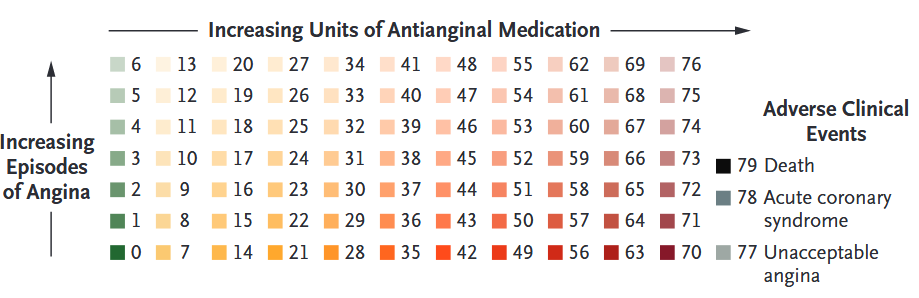
\includegraphics[width=6in]{rajkumar_et_al_outcome.png}
  \caption{``Angina Symptom Score'' ordinal outocome develped in
    \citep{rajkumarPlaceboControlledTrialPercutaneous2023}. This illustrates
    (1) complete tie-breaking (of units of antianginal medication by
    episodes of angina) and (2) overriding (of angina episodes and
      angina medication by adverse clinical events; of all other outcomes
  by death; etc.)}
  \label{fig:rajkumar_et_al_outcome}
\end{figure}

\begin{figure}
  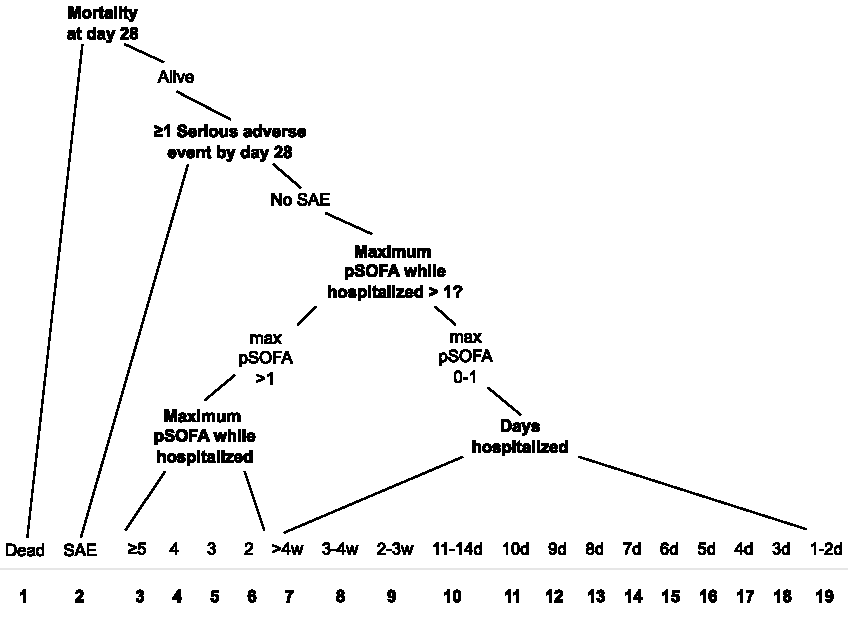
\includegraphics[width=5.5in]{passport_ordinal_outcome_tree.pdf}
  % 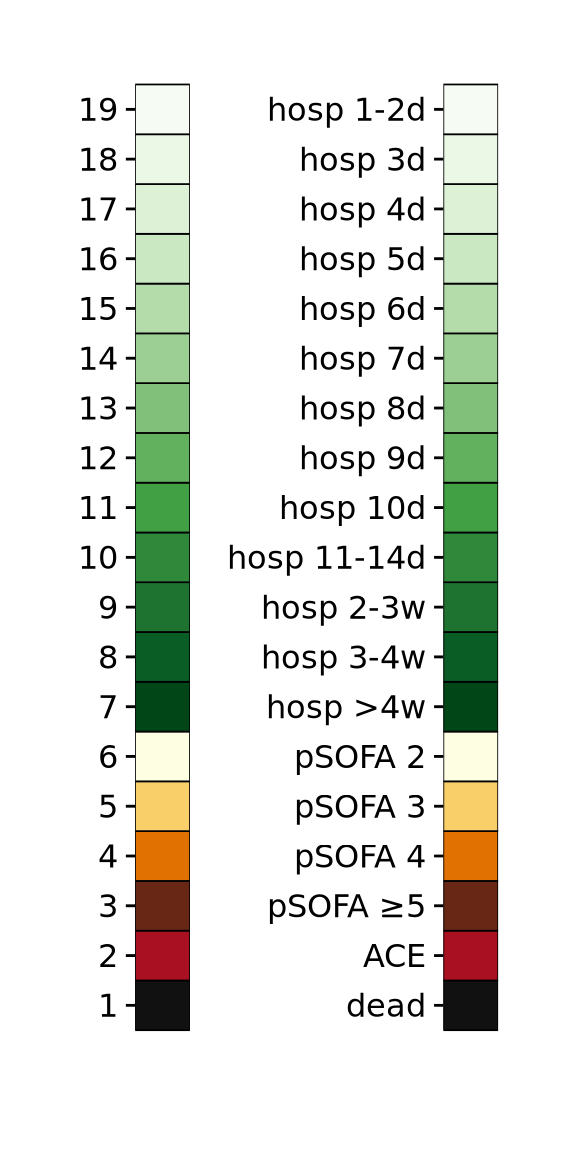
\includegraphics[width=1in]{passport_ordinal_outcome_colorbar.png}
  \caption{Ordinal outcome used in the planned PASSPORT adaptive
    platform trial. This illustrates (1) overriding (of hospital
    outcomes by pSOFA outcomes, etc.) but also (2) using tie-breaking
    to augment a ``state'' outcome (status at day 28) with
    longitudinal (maximum pSOFA while hospitalized) and time-to-event
    (days hospitalized)
  information}
  \label{fig:passport_outcome}
\end{figure}

\begin{figure}
  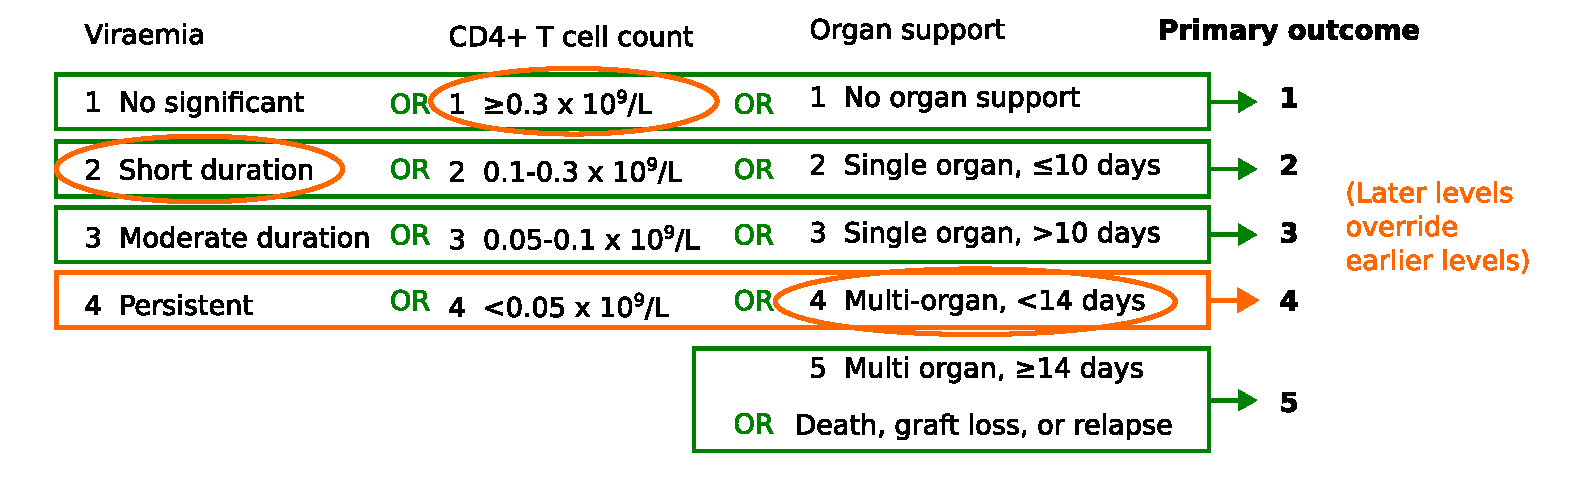
\includegraphics[width=7in]{parallel_composition_bandicoot.pdf}
  % 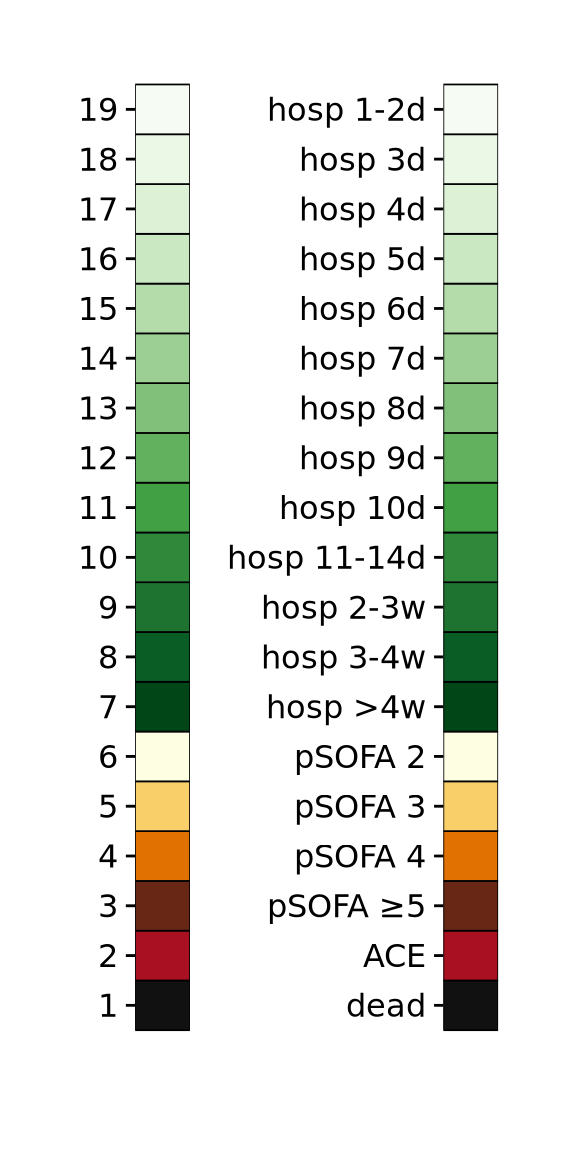
\includegraphics[width=1in]{passport_ordinal_outcome_colorbar.png}
  \caption{Ordinal outcome used in the planned BANDICOOT adaptive
    platform trial \citep{walkerCodesigningNovelOrdinal2025}.
  Illustrates \textbf{parallel composition} of component outcomes}
  \label{fig:parallel_bandicoot}
\end{figure}

\subsubsection{Tie breaking can augment a state outcome with longitudinal
information}

Distinguish between ``state'' and ``trajectory'' variables. State
variables summarize patient outcomes at a particular moment in time.
Trajectory variables, including times-to-event, summarize patient
state over a timecourse.

Trajectory and state variables can be incorporated into an ordinal outcome. For
example (from PASSPORT) ``worst pSOFA while hospitalized until day 28'' and
``length of hospitalization'', which are longitudinal variables (summary of a
trajectory), are combined with the day 28 state variable ``death''.

Incorporating trajectory variables into an ordinal outcome may seem unnatural.
But arguably most time-to-event analyses are in fact analyses of an
ordinal outcome. The Cox model for time-to-event data treats time as ordinal:
because (1) the baseline hazard is not modelled, (2) the model itself is
invariant to monotone rescalings of the time axis, and (3) the (partial)
likelihood (ignoring ties) depends only on the ranks of the data (i.e., is a
marginal likelihood). The Cox model is essentially an ordinal
stopping ratio model with complementary log-log link. (Perhaps a
difference is censoring.)

\subsubsection{Overriding can augment a continuous outcome}

For example overriding a continuous outcome by death. It would be
good to have an example of this.

\subsubsection{Precision and power depend mostly on the probability of the
largest category}

Theory of \citep{whiteheadSampleSizeCalculations1993} says that the relative
efficiency (variance) of an unadjusted treatment comparison using an ordinal
versus continuous outcome in the proportional odds model is given by $1 - \sum
\overline p_c^3$ where $\overline p_c$ is the marginal probability (averaged
over control and experimental groups) of outcome category $c$.

Efficiency is maximized at $1 - 1/C^2$ where $C$ is the total number of
categories when the probabilities are all equal: $\overline p_c = 1/C$.

We have simulation results and some math to show that the value of $\sum_c
\overline p_c^3$ is \emph{essentially a function of the largest category
probability} $\overline{p_{\max}} = \max \overline{p_c}$. See \ref{fig:p_max}
for an illustration.

\begin{figure}
  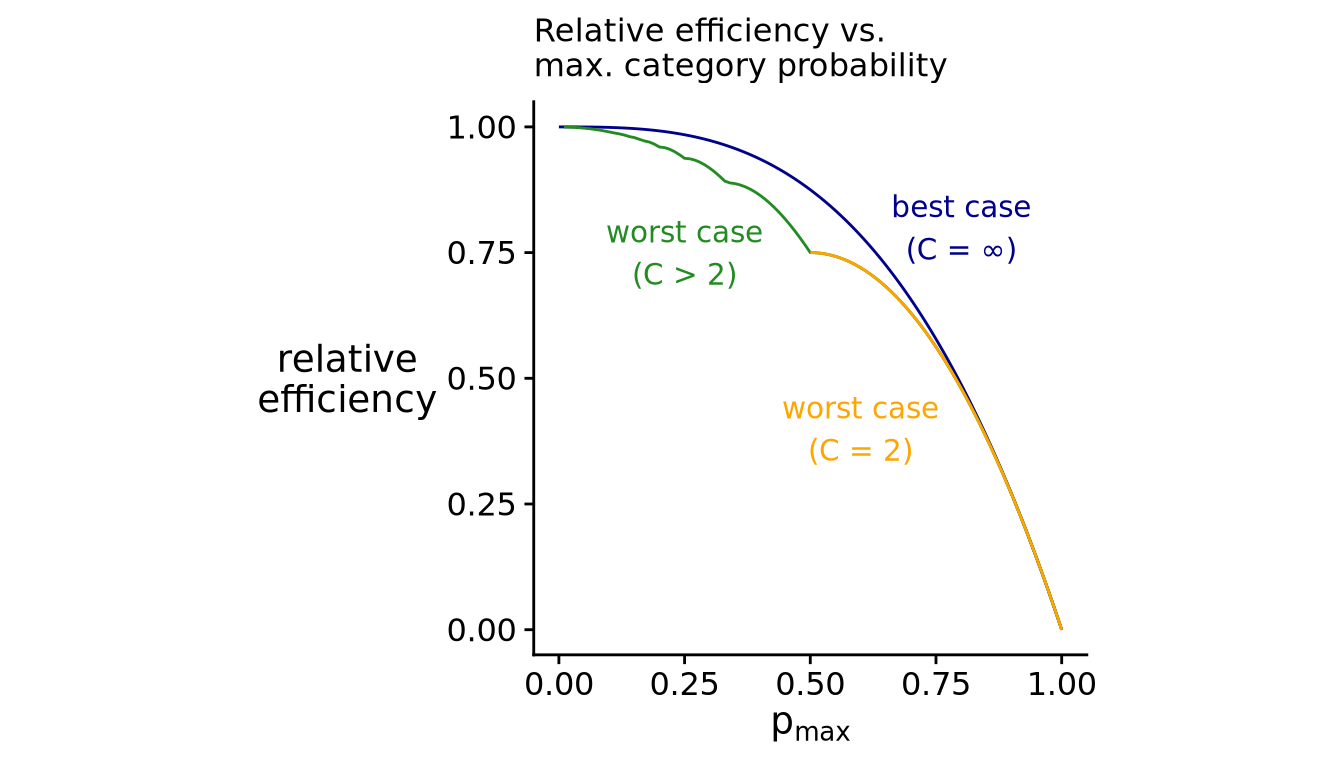
\includegraphics[width=6in]{p_max_controls_efficiency.png}
  \caption{Bounds on the relative efficiency of an ordinal outcome
    compared to its continuous counterpart as a function of the maximum
    category probability $p_\text{max}$. The upper bound (best case
    relative efficiency for a given $p_\text{max}$) is always achieved in the
    limit of infinitely many categories ($C = \infty$). The lower bound
    is always achieved when the number of categories is as small as
  possible for a given $p_\text{max}$.}
  \label{fig:p_max}
\end{figure}

Thus simple advice is: for statistical efficiency, try to make the proportion
of patients in the largest category small.

However a converse is: if the proportion of patients in the largest category is
small, not much is gained by tie-breaking.

\subsection{Coarsening and incorporating intercurrent events for validity}

\subsubsection{Coarsening to avoid directly comparing levels}

In the PASSPORT outcome (Figure \ref{fig:passport_outcome}), for
example, we include both digit
amputation and ECMO
any time within 28 days post-enrollment under the heading of
``adverse clinical events''.

Including these outcomes within the same level of an
ordinal outcome does not mean assuming that the two outcomes have the
\emph{same} utility. Rather it represents \emph{avoiding comparing}
their utilities. (This was something clinicians asked about more than once.)

\subsubsection{Coarsening for simplicity}

Too many levels can make it hard to directly compare meaningful
proportions/probabilities.

(It isn't really a problem for model fitting with modern software.)

Coarsening, including combining levels and replacing complete
tie-breaks with overrides, could help with this.

\subsubsection{Incorporating intercurrent events using tie-breaking
or overriding}

The intercurrent event could be (1) incorporated as a level (2) used
for tie-breaking or overriding.

This is a version of the ``composite strategy'' as described in e.g.
\citet{kahanEstimandsFrameworkPrimer2024}, but we expect it to yield
more efficiency than creating a \emph{binary} composite outcome.

\section{Choosing ordinal effect measures}

Goal: we want to compare two or more distributions over ordinal
outcomes with a single number. (Two distributions when comparing control and
experimental groups; more distributions when e.g. adjusting for covariates.)

In general this represents a loss of information. Let's say the
outcome has $C$ categories. Then the distribution in each
arm is specified by $C-1$ numbers (for the first $C-1$ probabilities,
  or cumulative logits, or stopping ratio logits--reflecting the
sum-to-1 constraint on probability distributions) and so the
\emph{difference} between the distributions is also specified by
$C-1$ numbers (for example the differences between the cumulative
logits, or logit stopping probabilities).

An effect measure thus represents a way to collapse these $C-1$
numbers into one.

It usually doesn't make sense to consider effect measures based on
numeric coding (e.g. difference in mean levels). This is adding
information that is not present in the basic ordinal structure.

\subsection{Model-based effect measures}

Model-based: common odds ratio; common stopping ratio or common continuation
ratio.

What they have in common: the effect measure is a byproduct of fitting a model
to the data.

The model typically assumes that a certain pattern holds in the outcome
distributions across groups. If the pattern holds, then the differences in
distributions can be described by a single number (with more than two groups,
$G-1$ numbers) instead of $(C-1)$ numbers.

\subsection{Model-free or nonparametric effect measures}

These are not based on a model (assumed pattern in the differences
between outcome distributions).

\subsubsection{Effect measures based on ``independent pairwise
comparison'' construction}

Probabilistic index/probability of
superiority, win ratio, win odds, etc. These predate win ratio and DOOR methods
\citep[e.g.][p.~14]{agrestiAnalysisOrdinalCategorical2010}.

Rather they are all be based on the ``\emph{pairs construction}'',
where we imagine independently sampling patients from the control and
treatment groups and considering ``wins'' ``ties'' and ``losses''
(corresponding to concordant and discordant pairs and ties in $y$
respectively). They can
also be \emph{estimated from data} using pairs of patients, but this
is not essential and they could also be estimated by fitting a
proportional odds model, for example (though they would not be a
simple function of a coefficient).

\subsubsection{Dichotomizing or comparing with a reference group}

\begin{itemize}
  \item Reducing to a binary outcome by picking a specific cutpoint,
    e.g. ``hospitalization or
    worse''. This is effectively using a binary outcome, but with the
    ordinal structure used to gain power if fitting a model.
  \item Reducing to a binary outcome using quantiles of a reference
    group; for example,
    ``worse than the median outcome under standard care''
  \item Ridit analysis
    \citep{brossHowUseRidit1958,agrestiAnalysisOrdinalCategorical2010,
    smithsonReceiverOperatingCharacteristic2023, jansenRiditAnalysisReview1984}
\end{itemize}

\subsection{Comparing model-based and nonparametric effect measures}

Both of these can be considered ``estimands'', insofar as we consider the
estimand associated with the model-based effect measures to be given by the
best-fitting model in the population.

Two classes of assumption violations for model-based effect measures
are \emph{magnitude}-heterogeneity across cutpoints (for example,
  effect of a treatment on hospital length of stay or worse is larger
  than its effect on
death on the relevant scale) and
\emph{sign}-heterogeneity
across cutpoints (failure of stochastic dominance -- for example,
treatment is beneficial for hospital length of stay, harmful for death).

Nonparametric effect measures may appear to be assumption-free. However

\begin{itemize}
  \item Assumptions don't need to hold exactly for the model-based
    effect measures to make sense
  \item In particular, if stochastic dominance holds, we can think of
    both model-based and nonparametric effect measures as
    testing the null hypothesis of no effect ``in a particular
    direction''. A weak interpretation of any particular
    effect measure
    is that it supplies this ``direction''.

    For example the Wilcoxon test is
    equivalent to the score test from fitting a proportional odds model.
    Thus fitting a proportional odds model (or any other model) has a
    valid null-testing
    interpretation even if proportional odds doesn't hold.
  \item Under failure of stochastic dominance (``sign
    heterogeneity''), \emph{neither} parametric nor nonparametric
    effect measures make sense, since it doesn't make sense to
    summarize effects by a single number. Need to dig into the
    cutpoint-specific effects.
  \item Model-free methods don't define a common scale for comparing
    more than two interventions. For example, model-free effect
    measures can be \emph{nontransitive}, so it's not clear how to
    use them in $\geq 2$-arm studies
  \item For the same reason, model-based methods have additional
    advantages, for example
    the possibility of adjustment for covariates.

    When additivity approximately holds, this yields a ``best of both
    worlds'' effect measure that is
    personalized (conditional) yet reportable as a single
    number.
\end{itemize}

Harrell critiques \citep{harrellOverviewCompositeOutcome2024,
harrellRareDegenerativeDiseases2024, harrellViewsCompositeOutcome}: mainly that
win probability etc. are \emph{relative measures}:

\begin{itemize}
  \item Comparable to Cohen's $d$ or $t$-statistic (difference in
    means divided by standard deviation or standard error) rather than
    difference in means: compare: standardized effect size of 0.2 vs.
    difference in means of 10 mmHg
  \item Affected by study inclusion criteria (why? probably needs to
    be fleshed out.)
\end{itemize}

Simulations show a typically very strong association between
proportional odds ratios and $c$-index
\citep{harrellViolationProportionalOdds2020}.

One point of view is that one would ``ideally'' analyze ordinal
outcomes by reporting the associated expected utilities \todo{cite Berry
talk; example of utility-weighted Rankin scale} and that since
existing ordinal methods supply such utilities implicitly why not
just supply them explicitly. A counterpoint is that the methods do not, in fact,
supply utilities implicitly.

We should distinguish between effect measures used for \emph{analysis} and for
\emph{reporting}. It may make sense to report the probabilistic index or a
single-cutpoint binary outcome even if the analysis is undertaken using a
proportional odds model.

\section{Situating win/DOOR/etc. methods in the broader context of ordinal
outcomes and effect measures}

Terms to define/distinguish:
\begin{itemize}
  \item Desirability of Outcome Ranking (outcome)
  \item Hierarchical composite endpoint (outcome)
  \item Prioritized outcomes (outcome)
  \item Win methods (win probability, win odds, win ratio) (effect
    measure; estimation methods)
  \item Generalized pairwise comparisons (effect measure)
\end{itemize}

These approaches implicitly \textbf{bundle together three different things}:
\begin{enumerate}
  \item Constructing an implicit ordinal outcome through
    complete tie-breaking
  \item Targeting a nonparametric effect measure defined via the
    ``pairs'' device (probabilistic
    index/win ratio/win odds/etc.)
  \item Estimating that effect measure in a nonparametric/flexible
    manner using pairs, often also with devices for accounting for censoring
\end{enumerate}

This paper is focused on first two steps.

Why is it useful to consider these three steps separately?

Consider some of the critiques of win methods in
\citet[e.g.~][]{ajufoFallaciesUsingWin2023}

\begin{itemize}
  \item Situating methods in their proper context can help
    trialists make informed choices among them
  \item Win methods can make use of
    plots and diagnostics for general ordinal outcomes, e.g.
    comparative CDF plots.
  \item Ordinal regression models can use win methods for model checking; it is
    also possible to present a model-based win effect measure alongside a common
    odds ratio for example.
  \item The outcomes \emph{implicitly} constructed using
    DOOR and win methods may contain many levels, and may contain
    levels where an
    effect is not so meaningful (e.g. time-to-death when the followup time is
    short). By \emph{explicitly} constructing the associated ordinal outcome one
    might be forced to be more aware of this
  \item What is a reasonable win
    analysis of a specific component score? From the traditional
    ordinal endpoint
    school of thought what would make most sense is to \emph{only
      tie-break for the
    lowest and highest levels of that score}, and e.g. plot eCDFs of this new
    variable. Is this what the plots do that break down wins and losses by
    component score?
\end{itemize}

Disadvantages of generalized pairwise comparison approaches
\begin{itemize}
  \item Inherited from downsides of complete tiebreaking
  \item Inherited from downsides of nonparametric/pairwise effect measures
  \item Regression methods exist, but are newer and less battle-tested
\end{itemize}

\todo{``Partial credit'' analysis?}

\section{Conclusions}

\newpage

\section{Bibliography}

\printbibliography

\end{document}
